\documentclass[a4paper,12pt]{article}
\usepackage[utf8]{inputenc}
\usepackage{amsmath}
\usepackage{amssymb}
\usepackage{stmaryrd}
\usepackage{geometry}
\usepackage{enumitem}
\usepackage{fancyhdr}
\usepackage{tikz}
\usepackage{amsopn}

\newcommand{\sem}[1]{[\![ #1 ]\!]}

\geometry{margin=1in}
\pagestyle{fancy}
\fancyhf{}
\lhead{Dataflow Analysis: Monotone Frameworks, Widening \& Path Sensitivity}

\begin{document}

\section*{Introduction (2 Minutes)}

Today I will present the core concepts of \textbf{Dataflow Analysis} using \textbf{Monotone Frameworks}. We will start by establishing the general mathematical structure that allows us to solve flow-sensitive problems like Constant Propagation or Liveness Analysis. \\
\\ However, standard frameworks have limitations. Specifically, they require lattices of finite height to guarantee termination, and they often ignore the specific path taken through the control flow graph. \\
\\
Therefore, in the second half of the presentation, I will introduce \textbf{Widening and Narrowing} to handle infinite lattices (like Interval Analysis) and \textbf{Path Sensitivity} to handle correlated branches. \\
\\ \textbf{Whiteboard Action:}
\begin{itemize}
    \item Write the title: \textbf{Dataflow Analysis}.
    \item Draw a simple CFG node $v$ with predecessors $w_1, w_2$.
    \begin{center}
        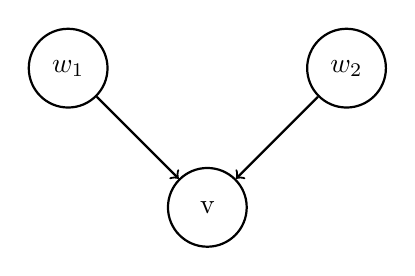
\begin{tikzpicture}[
        node distance=2.5cm,
        every node/.style={circle, draw, minimum size=1cm, thick}
        ]
        \node (v) {v};
        \node[above left of=v] (w1) {$w_1$};
        \node[above right of=v] (w2) {$w_2$};
        \draw[->, thick] (w1) -- (v);
        \draw[->, thick] (w2) -- (v);
        \end{tikzpicture}
    \end{center}
\end{itemize}

\hrule

\section*{Part 1: Monotone Frameworks (Detailed Breakdown)}

To perform dataflow analysis systematically, we use a \textbf{Monotone Framework}. A framework is essentially a pair: a Control Flow Graph (CFG) representing our program, and a \textbf{Complete Lattice} $L$ representing the abstract information we want to track. \\
\\ For every node $v$ in the CFG, we assign a \textbf{constraint variable}, denoted as $\sem{v}$. This variable holds an element of our lattice $L$—an 'abstract state'—associated with that program point. \\
\\ The core of the analysis is defining how this information flows and changes. We do this by setting up a \textbf{Dataflow Constraint} for every node. The constraint equation generally looks like this:

\paragraph{Whiteboard Action:}
\begin{itemize}
    \item Write: $\sem{v} = f_v(JOIN(v))$ 
\end{itemize}
This equation has two distinct parts that do very different jobs: the \textbf{JOIN} operation and the \textbf{Transfer Function} ($f_v$). \\
\\ First, let's look at \textbf{JOIN}.
In a control flow graph, execution paths merge. We might arrive at node $v$ from multiple different places. Since we are doing static analysis, we must be conservative and consider \textit{all} possible incoming paths. The JOIN operation combines the abstract states from these neighbors into a single, safe state. \\
\\ The definition of JOIN depends entirely on the \textbf{direction} of our analysis:

\paragraph{Whiteboard Action:}
\begin{itemize}
    \item Write:
    \begin{itemize}
        \item \textbf{Forward Analysis:} $JOIN(v) = \bigsqcup_{w \in pred(v)} \sem{w}$ (Combine information from the past).
        \item \textbf{Backward Analysis:} $JOIN(v) = \bigsqcup_{w \in succ(v)} \sem{w}$ (Combine information from the future).
    \end{itemize}
\end{itemize}
Once we have joined the incoming information, we apply the \textbf{Transfer Function}, denoted as $f_v$ (or sometimes $t_v$). \\
\\ The Transfer Function models the \textit{semantics} of the statement at node $v$. It specifies how the execution of that specific statement transforms the abstract state. \\
\\ For example, if we are doing Sign Analysis and node $v$ is the statement `x = -5`:
\begin{itemize}
    \item The JOIN operation tells us the state of the world right before we execute the statement.
    \item The Transfer Function $f_v$ takes that state and updates it to reflect that `x` is now definitely Negative.
\end{itemize}
So, in summary: JOIN merges the paths to get us to the node, and the Transfer Function calculates the effect of the node itself. \\
\\ We also distinguish between \textbf{May} and \textbf{Must} analysis based on the lattice ordering and the join operator:
\begin{enumerate}
    \item \textbf{May Analysis} (e.g., Liveness): Uses union ($\cup$) as the join. It over-approximates.
    \item \textbf{Must Analysis} (e.g., Available Expressions): Uses intersection ($\cap$) as the join. It under-approximates.
\end{enumerate}
If the lattice $L$ has finite height and the functions $f_v$ are \textbf{monotone}, we can use Kleene's Fixed-Point Theorem. We simply iterate from the bottom element $\perp$ until the values stabilize to the least fixed point, $lfp(f)$. \\
\\ \textbf{Whiteboard Action:}
\begin{itemize}
    \item Draw the classification table:
    \begin{center}
    \begin{tabular}{|c|c|c|}
    \hline
     & Forward & Backward \\
    \hline
    May ($\cup$) & Reaching Defs & Live Vars \\
    \hline
    Must ($\cap$) & Avail. Expr & Very Busy Expr \\
    \hline
    \end{tabular}
    \end{center}
\end{itemize}

\hrule

\section*{Part 2: Widening and Narrowing (5 Minutes)}

The framework I just described works perfectly if our lattice has \textit{finite height}. But what if we want to track ranges of integers? We use the \textbf{Interval Lattice}:
$$ Interval = lift(\{ [l, h] \mid l, h \in N \wedge l \le h \}) $$
Here, $N$ includes $-\infty$ and $\infty$. The problem is that this lattice has \textbf{infinite height}.

\paragraph{Whiteboard Action:}
\begin{itemize}
    \item Draw the infinite chain: $[0,0] \sqsubseteq [0,1] \sqsubseteq [0,2] \dots$ 
\end{itemize}
Consider this example from the course book:
\begin{verbatim}
y = 0; x = 7; x = x + 1;
while(input) {
    x = 7; x = x + 1;
    y = y + 1;
}
\end{verbatim}
Without special handling, the analysis of `y` inside the loop would produce the sequence $[0,0], [0,1], [0,2], \dots$ and never terminate. \\
\\ To fix this, we use \textbf{Widening} ($\nabla$). We introduce a set of constants $B$ (e.g., $\{-\infty, 0, 1, 7, \infty\}$). If a bound is unstable, we widen it immediately to the next value in $B$.
For our example, `y` jumps from $[0,1]$ directly to $[0, \infty]$. \\
\\ This guarantees termination, but it overshoots. In this example, widening might conclude that $x$ is $[7, \infty]$, which is safe, but very imprecise because we can see that $x$ is always 8 inside the loop. \\ 
\\ To recover this precision, we use \textbf{Narrowing}. This is where we must understand the math.\\
\\ The result of widening, let's call it $f_\nabla$, is a \textbf{safe approximation}. Mathematically, this means two things:
1. It is above the least fixed point: $lfp(f) \sqsubseteq f_\nabla$.
2. It is a \textit{post-fixed point}: $f(f_\nabla) \sqsubseteq f_\nabla$. \\
\\ Because of property \#2, if we apply the transfer function $f$ one more time to our result, we get a value $f(f_\nabla)$ that is \textbf{smaller} (more precise) than what we started with. \\
\\ But is it still safe? Yes, because our transfer function $f$ is \textbf{monotone}. Since $lfp(f) \sqsubseteq f_\nabla$, applying $f$ to both sides implies $f(lfp(f)) \sqsubseteq f(f_\nabla)$. Since $f(lfp(f))$ is just $lfp(f)$, we prove that our new result is still a valid upper bound. \\
\\ In our example, applying narrowing brings $x$ from $[7, \infty]$ back down to $[8,8]$, perfectly restoring the lost information.''

\paragraph{Whiteboard Action:}
\begin{itemize}
    \item Write the Narrowing Logic:
    $$ \underbrace{lfp(f) \sqsubseteq f(f_\nabla)}_{\text{Still Safe}} \sqsubseteq \underbrace{f_\nabla}_{\text{More Precise}} $$
    \item Show the Example Result:
    $$ x: [7, \infty] \xrightarrow{\text{Narrowing}} [8, 8] $$
\end{itemize}

\hrule

\section*{Path Sensitivity (4 Minutes)}

Standard monotone frameworks are \textbf{path-insensitive}. They merge information from all branches using the Join operator ($\bigsqcup$), losing the correlation between variables. \\
\\Consider a case where we open a file only if a \texttt{flag} is set, and close it only if the \texttt{flag} is set. A standard analysis merges the paths and might conclude we are closing a file that might not be open. \\
\\To fix this, we introduce \textbf{Path Sensitivity}. We can do this in two ways:

\paragraph{1. Control Sensitivity (Assertions)}
We can explicitly model conditions using an \texttt{assert(E)} statement. If we have \texttt{if (x > 0)}, we insert \texttt{assert(x > 0)} in the true branch and \texttt{assert(!(x > 0))} in the false branch.
In Interval Analysis, \texttt{assert(x > 0)} refines the interval of $x$. If $x$ was $[-\infty, \infty]$, it becomes $[1, \infty]$ in that branch.

\paragraph{2. Relational Analysis (Path Contexts)}
For stronger properties (like the file-flag correlation), we use a \textbf{Relational Analysis}.
We replace our lattice $L$ with a map lattice:
$$ L' = Path \rightarrow L $$
Here, $Path$ is a set of path contexts (e.g., predicates like $\{flag=0, flag \neq 0\}$).
Instead of one abstract state per node, we maintain a separate state for every context. \\
\\ \textbf{Whiteboard Action:}
\begin{itemize}
    \item Write lattice def: $L' = Path \rightarrow \mathcal{P}(\{open, closed\})$
    \item Example constraint for \texttt{open()}:
    $$ \sem{open()} = \lambda p . \{open\} $$
    \item Example constraint for \texttt{flag=0}:
    $$ \sem{flag=0} = [flag=0 \mapsto \bigcup_{p} JOIN(v)(p), \quad flag \neq 0 \mapsto \emptyset] $$
\end{itemize}
By separating the dataflow based on the `flag` context, we can prove that in the `flag $\neq$ 0` context, the file is open, and in the `flag = 0` context, the file is closed. This solves the precision problem. \\

\hrule

\section*{Conclusion ($<$ 1 Minute)}

In summary, Monotone Frameworks provide the theoretical foundation for static analysis using lattices and fixed-point algorithms.
\begin{itemize}
    \item When the lattice height is infinite, we apply \textbf{Widening} to ensure termination and \textbf{Narrowing} to restore precision.
    \item When control flow correlations matter, we use \textbf{Path Sensitivity} (via assertions or relational path contexts) to distinguish feasible execution paths.
\end{itemize}
Thank you. I am happy to take any questions.

\end{document}